%%%%%%%%%%%%%%%%%%%%%%%%%%%%%%%%%%%%%%%%%%%%%%%%%%%%%%
%%%%%%%%%%%%%%%%% PAGE DE GARDE  %%%%%%%%%%%%%%%%%%%%%
%%%%%%%%%%%%%%%%%%%%%%%%%%%%%%%%%%%%%%%%%%%%%%%%%%%%%%

%Une commande sembleble � \rlap ou \llap, mais centrant son argument
\def\clap#1{\hbox to 0pt{\hss #1\hss}}%
%Une commande centrant son contenu (� utiliser en mode vertical)
\def\ligne#1{%
  \hbox to \hsize{%
    \vbox{\centering #1}}}%
%Une comande qui met son premier argument � gauche, le second au 
%milieu et le dernier � droite, la premi�re ligne ce chacune de ces
%trois boites co�ncidant
\def\haut#1#2#3{%
  \hbox to \hsize{%
    \rlap{\vtop{\raggedright #1}}%
    \hss
    \clap{\vtop{\centering #2}}%
    \hss
    \llap{\vtop{\raggedleft #3}}}}%
%Idem, mais cette fois-ci, c'est la derni�re ligne
\def\bas#1#2#3{%
  \hbox to \hsize{%
    \rlap{\vbox{\raggedright #1}}%
    \hss
    \clap{\vbox{\centering #2}}%
    \hss
    \llap{\vbox{\raggedleft #3}}}}%
%La commande \maketitle
\def\maketitle{%
  \thispagestyle{empty}\vbox to \vsize{%
    \haut{}{\@blurb}{}
    \vspace{3cm}
   
    %\vfill
    \begin{center}\leavevmode
    	\normalfont
    	{\raggedleft \@author\par}%
    	%\thickhrulefill\par
    	\vspace{20mm} \hrule height 2pt 
    	{\huge\center \textbf{\@title}}%
    	\vspace{5mm} \hrule height 2pt \vspace{5mm}
	\vfill
    	\vskip 1cm
    	{\LARGE\center\textsc{}}
    	\vskip 2cm

    	
    \end{center}% 
    \vskip 1cm
    }%
  \cleardoublepage
  }

%Les commandes permettant de d�finir la date, le lieu, etc.
\def\date#1{\def\@date{#1}}
\def\author#1{\def\@author{#1}}
\def\title#1{\def\@title{#1}}
\def\location#1{\def\@location{#1}}
\def\blurb#1{\def\@blurb{#1}}
\def\email#1{\def\@email{#1}}
%Valeurs par d�faut
\date{\today}
\author{}
\title{}
\location{Marseille}
\blurb{}
\email{patrick.chaumet@fresnel.fr}
\makeatother
%
%%%%%%%%%%%%%%%%%%%%%%%%%%%%%%%%%%%%%%%%%%%%%%%%%%%%%%%%%%%%%%%%%%%%
\blurb{
\begin{center}
\parpic{
%\resizebox{160mm}{!}{\includegraphics{logofac.eps}}
}
\picskip{0}
\end{center}
 {\huge \textsc{Institut Fresnel}} 
}

\title{IF-DDA \\ \vspace{5mm} \textsc{Idiot Friendly-Discrete Dipole
    Approximation}\\ \vspace{5mm} {\Large version : 0.6.5} }
\author{\center{\LARGE \textsc{Patrick
      C. Chaumet} \\ \vspace{5mm} \textsc{Daniel Sentenac} \\
    \vspace{5mm} \textsc{Anne Sentenac}}}

\atxy(3cm,17cm){\resizebox{140mm}{!}{\includegraphics{schemamic.eps}}}



\email{patrick.chaumet@fresnel.fr}
\date{}


\newpage{\pagestyle{empty}\cleardoublepage}


\maketitle
\newpage{\pagestyle{empty}\cleardoublepage}